% ----------------------------------------------------------------------- %
% Arquivo: cap3.tex
% ----------------------------------------------------------------------- %
\chapter{Federação CAFe}
\label{c_cap3}

Em Julho de 2007 a RNP com a colaboração das instituições Cefet-MG, UFC, UFF, UFMG, e UFRGS, dentro do escopo do projeto e-AA: Infraestrutura de Autenticação  e Autorização Eletrônica tinha como objetivo criar condições necessárias para a implantação de uma comunidade acadêmica federada no Brasil. Uma federação acadêmica envolve instituições de ensino e pesquisa e permite que as pessoas vinculadas a estas instituições compartilhem informações e recursos e tenham acesso a serviços restritos, usando o vínculo institucional como critério básico para esse compartilhamento \cite{moreira:11}. A partir destes esforços surgiu a \acf{CAFe}.

A CAFe tem como objetivo congregar todas as universidades e instituições de pesquisa brasileiras. A metodologia adotada para construção da infraestrutura básica de federação consiste na utilização de padrões e soluções de software já disponíveis e adotados por outras federações, e da implementação e experimentação de ferramentas auxiliares para apoiar a implantação de provedores de identidades e de serviços. O projeto de criação da Federação CAFe inclui ainda o estudo, a proposição, a análise e a validação de políticas para regular o funcionamento da federação \cite{moreira:11}.

\section{Como funciona}
\label{s_c3_funciona}

As instituições pertencentes à CAFe podem atuar como provedores de identidade (IdP) ou como provedores de serviço (SP), ou ainda podem ter ambos os provedores dentro das suas dependências. As organizações usuárias da RNP que atuam como provedores de identidade têm atualmente um subsídio completo no preço associado ao uso do serviço da CAFe. Além disso, nenhum dos acordos atuais prevê qualquer custo para os provedores de serviço. A RNP é responsável pela gestão do serviço e por manter o repositório centralizado com dados sobre integrantes da federação \cite{rnp:13}.

A CAFe possibilita que cada usuário tenha uma conta única em sua instituição de origem, válida para todos os serviços oferecidos à federação, eliminando a necessidade de múltiplas senhas de acesso e processos de cadastramento. A relação de confiança entre instituições participantes da Federação permite que o usuário se autentique unicamente em sua instituição de origem, que fornece as garantias de autenticidade e credibilidade necessárias às demais \cite{rnp:13}.

Outro aspecto positivo é o controle sobre a privacidade dos dados. Ao invés de ter um cadastro individual em cada serviço, a federação permite que o provedor de identidade forneça ao provedor de serviço apenas o mínimo de informação necessária para o controle de autorizações. Isto pode variar da simples garantia de que aquele usuário é reconhecido e autenticado pela instituição até informações sobre seu status ou tempo de serviço junto a essa instituição. Os acordos firmados pelos provedores de serviço com a CAFe garantem que os dados serão usados apenas para os fins combinados\footnote{http://portal.rnp.br/web/servicos/beneficios}.

Diversos países já têm federações em funcionamento ou em implantação. Dentro das redes de instituições de ensino, os serviços de ensino a distância e atividades de colaboração estão entre os maiores beneficiários das infraestruturas oferecidas por federações \cite{rnp:13}.

\section{Serviços disponíveis}
\label{s_c3_servicos}

Alguns serviços disponíveis através da CAFe são:

\begin{itemize}
 \item video@RNP -- O portal de Vídeo Digital da RNP agrega três diferentes serviços (Vídeo Sob Demanda, Transmissão de Vídeo ao Vivo e Transmissão de Sinal de TV) e se integra ao conteúdo do serviço Videoaula@RNP;
 \item JEMS -- O Journal and Event Management System (JEMS) é um sistema para submissão, revisão, discussão e seleção de artigos para eventos científicos da Sociedade Brasileira de Computação (SBC), mantido pela Universidade Federal do Rio Grande do Sul (UFRGS). Seu principal objetivo é disponibilizar para acadêmicos participantes de eventos da SBC uma infraestrutura para envio de artigos e resumos para avaliação. Assim, é possível a análise de tais documentos por parte da organização do evento e a decisão de quais deles serão selecionados para participação;
 \item GENI -- O \textit{Global Environment for Network Innovations} (GENI\footnote{https://portal.geni.net/}) é um portal de infraestrutura de pesquisa patrocinado pela National Science Foundation, órgão dos Estados Unidos de fomento ao desenvolvimento científico. O portal disponibiliza um ambiente laboratorial para redes e sistemas distribuídos para ensino e pesquisa com múltiplos testbeds. O laboratório virtual possibilita pesquisas sobre o futuro das redes de grande porte, criando oportunidades de compreensão, inovação e transformação das redes globais e suas interações com a sociedade;
 \item RedCLARA -- Os serviços que operam sobre a infraestrutura de Internet Avançada de RedCLARA\footnote{http://www.redclara.net/index.php} são destinados a promover o desenvolvimento de iniciativas de colaboração científica e acadêmica na América Latina, oportunidades reais para pesquisadores, cientistas e acadêmicos da região;
 \item Gisela -- O Gisela Science Gateway é um portal de aplicações científicas do projeto Grid Initiatives for e-Science virtual Communities in Europe and Latin America (GISELA), que funciona como uma interface para um ambiente de grid;
 \item Atlases -- O Atlases é uma biblioteca de imagens de patologia em alta resolução. É voltado para estudantes de Medicina e profissionais da área médica;
 \item PADBR -- A grade computacional PADBR oferece acesso integrado aos recursos de alto desempenho distribuídos geograficamente entre os Centros Nacionais de Processamento de Alto Desempenho (CENAPADs) geograficamente distribuídos. São nove unidades, operadas respectivamente pela UFRGS, UFMG, UFC, UNICAMP, UFRJ, UFPE, INPE, INPA e LNCC. Esse último coordena o sistema por delegação do Ministério da Ciência, Tecnologia e Inovação (MCTI).
\end{itemize}

Todos os serviços descritos acima estão disponíveis para acesso gratuito. Além destes, muitos outros serviços podem ser utilizados através do acesso pela CAFe. Uma lista de serviços pode ser vista no \textit{site} da CAFe, em serviços disponíveis\footnote{http://portal.rnp.br/web/servicos/servicos-disponiveis}

\section{Acordos internacionais}
\label{s_c3_acordos}

A disponibilização, ou criação de novas, infraestruturas de autenticação e autorização federadas para as suas comunidades acadêmicas está se tornando uma prática comum em vários países. O próprio Shibboleth, software utilizado na CAFe, foi desenvolvido pela Internet2 para dar suporte à criação da Federação InCommon\footnote{http://www.incommonfederation.org/}. Tipicamente, as iniciativas de criação de infraestruturas federadas são coordenadas pelas redes nacionais de ensino e pesquisa, \ac{NREN}, como a RNP. A CAFe se tornou um projeto pioneiro no Brasil e alcançou acordos internacionais, permitindo e à integração entre diferentes federações do Mundo \cite{rnp:13}.

\subsection{EduGAIN}
\label{ss_c3_edugain}

A Comunidade Acadêmica Federada (CAFe) integra, desde dezembro de 2012, o serviço eduGAIN\footnote{http://www.geant.net/service/edugain/pages/home.aspx}, que reúne, em uma rede de confiança, as federações de gestão de identidade sócias da GÉANT\footnote{http://www.geant.net/pages/home.aspx} (Rede de pesquisa pan-européia). A organização é uma rede de alta capacidade que engloba mais de três mil instituições de ensino e pesquisa em 32 países, através de 28 redes nacionais e regionais de ensino e pesquisa.

\begin{figure}[!htpb]
 \centering
 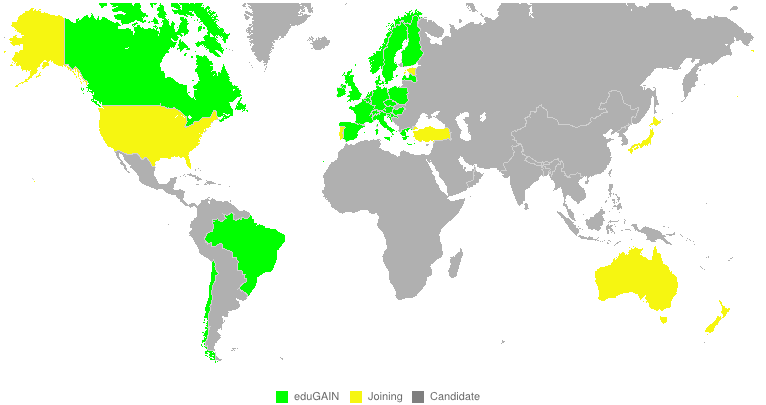
\includegraphics[width=1\textwidth]{figuras/edugain2.png}
 \caption{Mapa de países com federações participantes da EduGAIN. Fonte: EduGAIN (http://edugain.org/technical/status.php)}
 \label{fig_6}
\end{figure}

Além do Brasil, representado pela CAFe, fazem parte da eduGAIN federações da Croácia, Finlândia, Hungria, Itália, Noruega, Espanha, Suécia e Suíça. Constam também na lista de candidatos a integrar a confederação os seguintes países: República Tcheca, França, Alemanha, Grécia, Letônia e Holanda. A CAFe foi, portanto, a primeira federação das Américas a fazer parte desta rede de confiança.

O principal benefício para os clientes da CAFe é a possibilidade de utilizar os diversos serviços disponibilizados pelas inúmeras organizações que integram eduGAIN.

\subsection{REFEDS}

Desde março de 2011, a CAFe integra o mapa das federações de identidade mundiais de educação e pesquisa mantido pela Research and Education Federations (REFEDS)\footnote{http://www.terena.org/activities/refeds}.

\begin{figure}[!htpb]
 \centering
 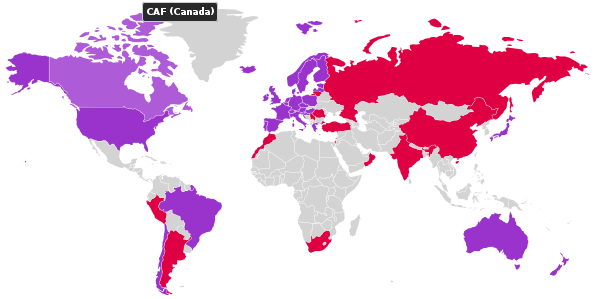
\includegraphics[width=1\textwidth]{figuras/cafe-refeds.png}
 \caption{Mapa de países com federações participantes da REFEDS. Fonte: REFEDS (https://refeds.org/resources/)}
 \label{fig_7}
\end{figure}

Assim, a CAFe se tornou a primeira federação da América Latina a ser reconhecida internacionalmente pela iniciativa, gerenciada pela \ac{TERENA}\footnote{http://www.terena.org/}, que articula as necessidades de federações de identidade para educação e pesquisa em todo o mundo.

Os participantes da REFEDS compartilham o interesse de desenvolver tecnologias, políticas e processos de gestão de identidade. Muitos destes representam redes nacionais de ensino e pesquisa, \ac{NREN}, como é o caso da RNP.